\begin{frame}{Lepditau Neural network}
    \begin{columns}
        \begin{column}{0.5\textwidth}
            \begin{figure}
                \centering
                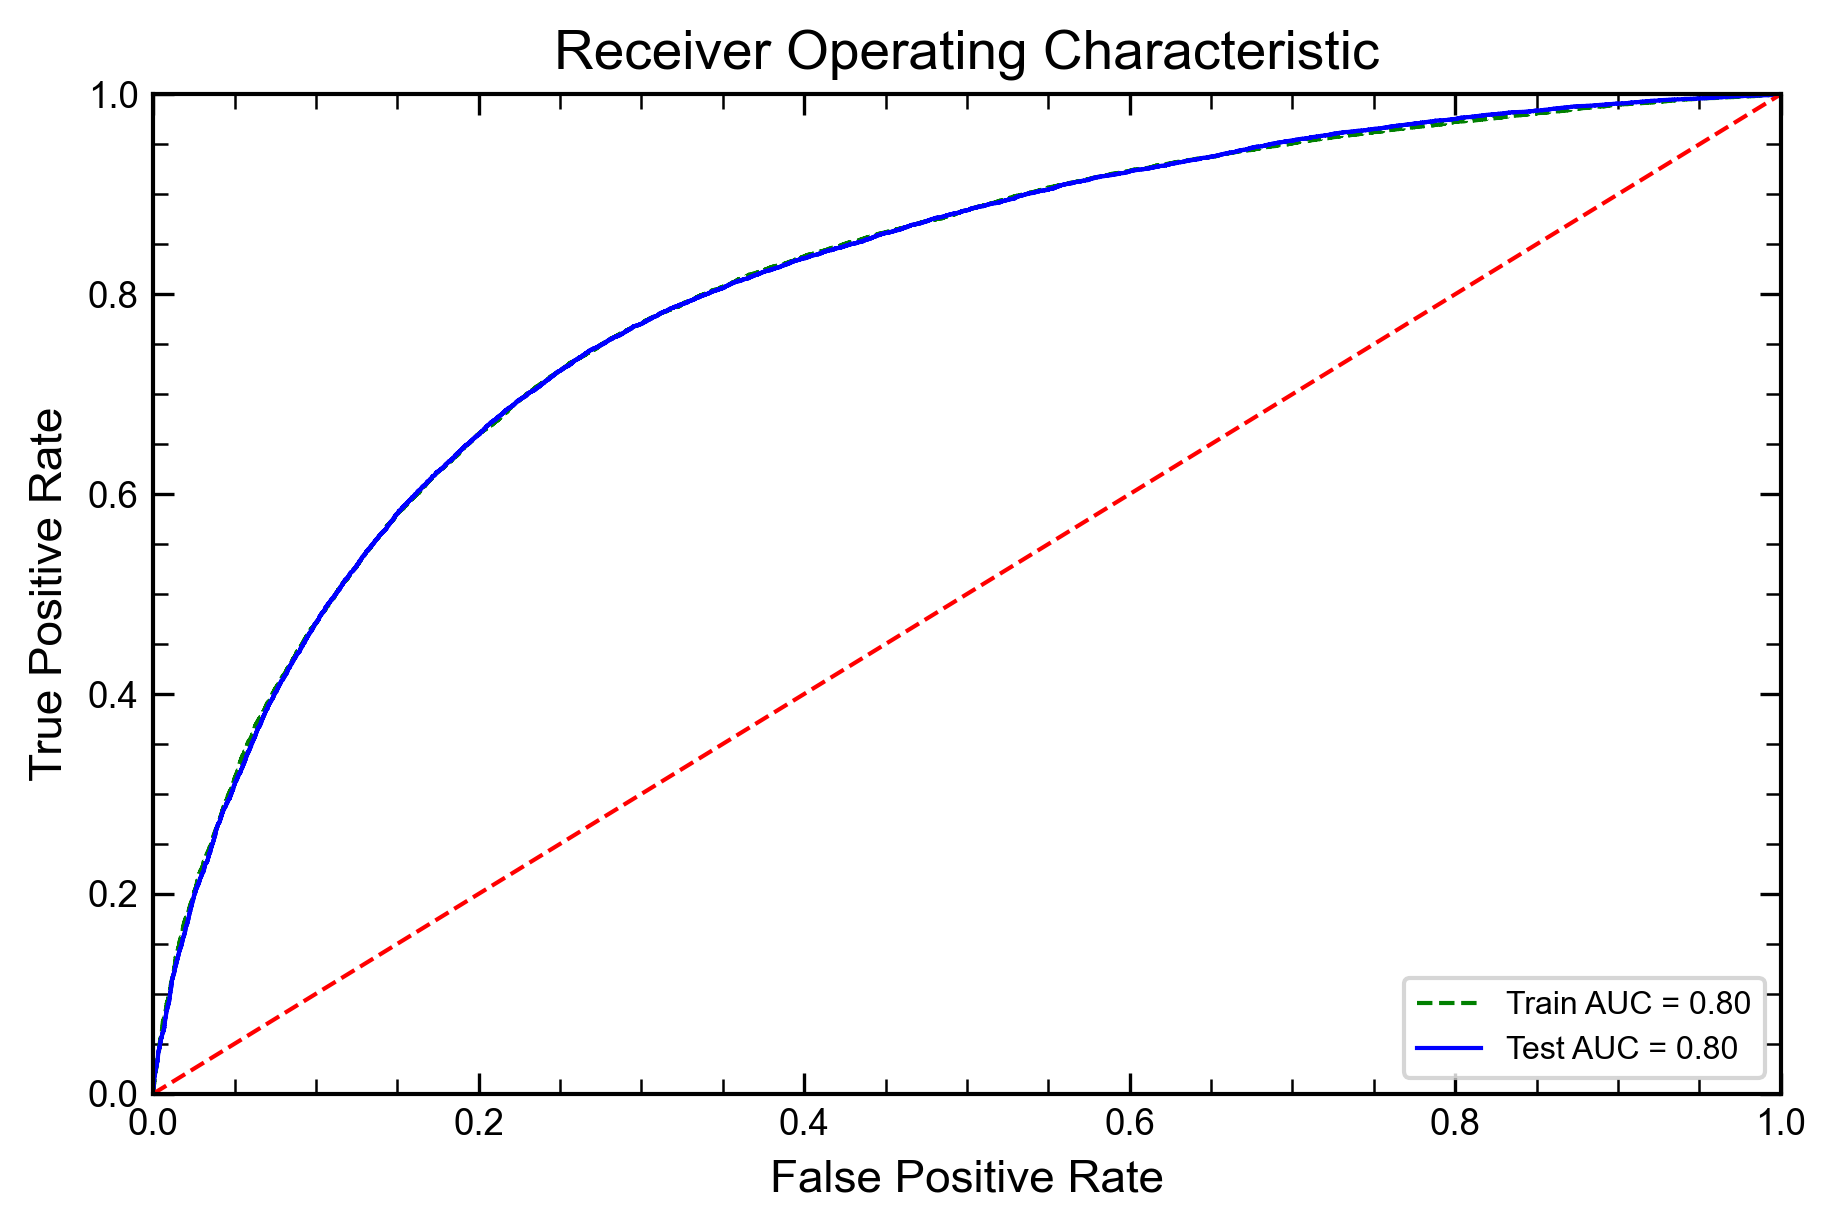
\includegraphics[width=0.8\textwidth]{hadhad_ROC}    
            \end{figure}
            \vspace{-0.35cm}
            \begin{figure}
                \centering
                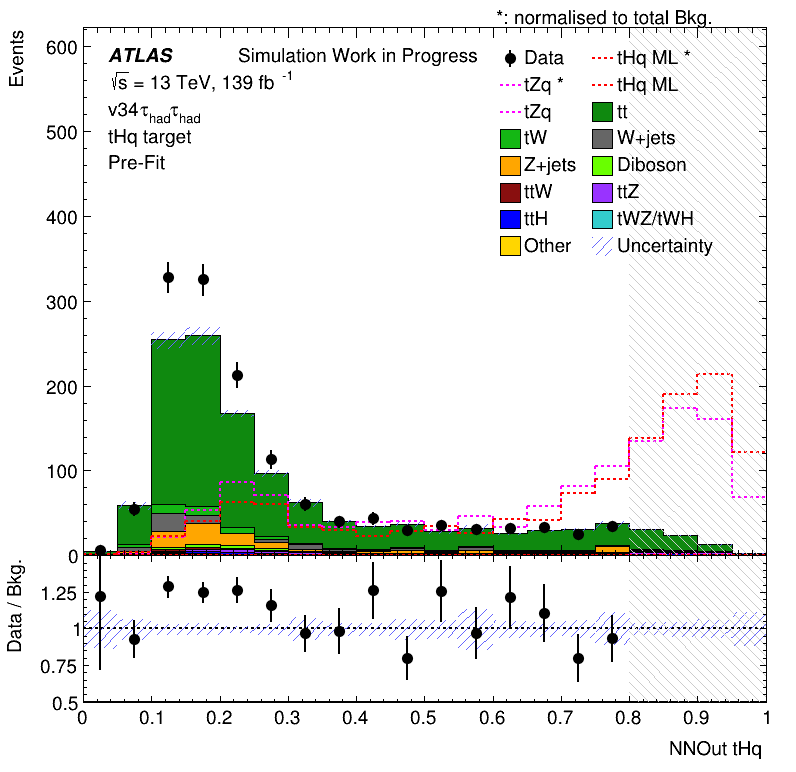
\includegraphics[width=0.8\textwidth]{NNOut_hadhad}    
            \end{figure}
        \end{column}
        \begin{column}{0.5\textwidth}
            \vspace{-0.25cm}
            \begin{block}{Setup}
                \begin{itemize}
                    \item Optimisation: Evolutionary + grid search
                    \item Model: Categorical (currently binary for v34)
                    \item Variables: final state kinematics
                    \item Currently performance problems for v34
                    \item Train on absolute, predict on full weights
                \end{itemize}
            \end{block}
            \vspace{-0.45cm}
            \begin{block}{Plans}
                \begin{itemize}
                    \item Validate categorical setup in lepditau
                    \item Rerun the optimisation for v34
                    \item Rank and test variables
                \end{itemize} 
             \end{block}
        \end{column}
    \end{columns}
\end{frame}

\begin{frame}{Dileptau Neural network}
    \begin{columns}
        \begin{column}{0.5\textwidth}
            \begin{figure}
                \centering
                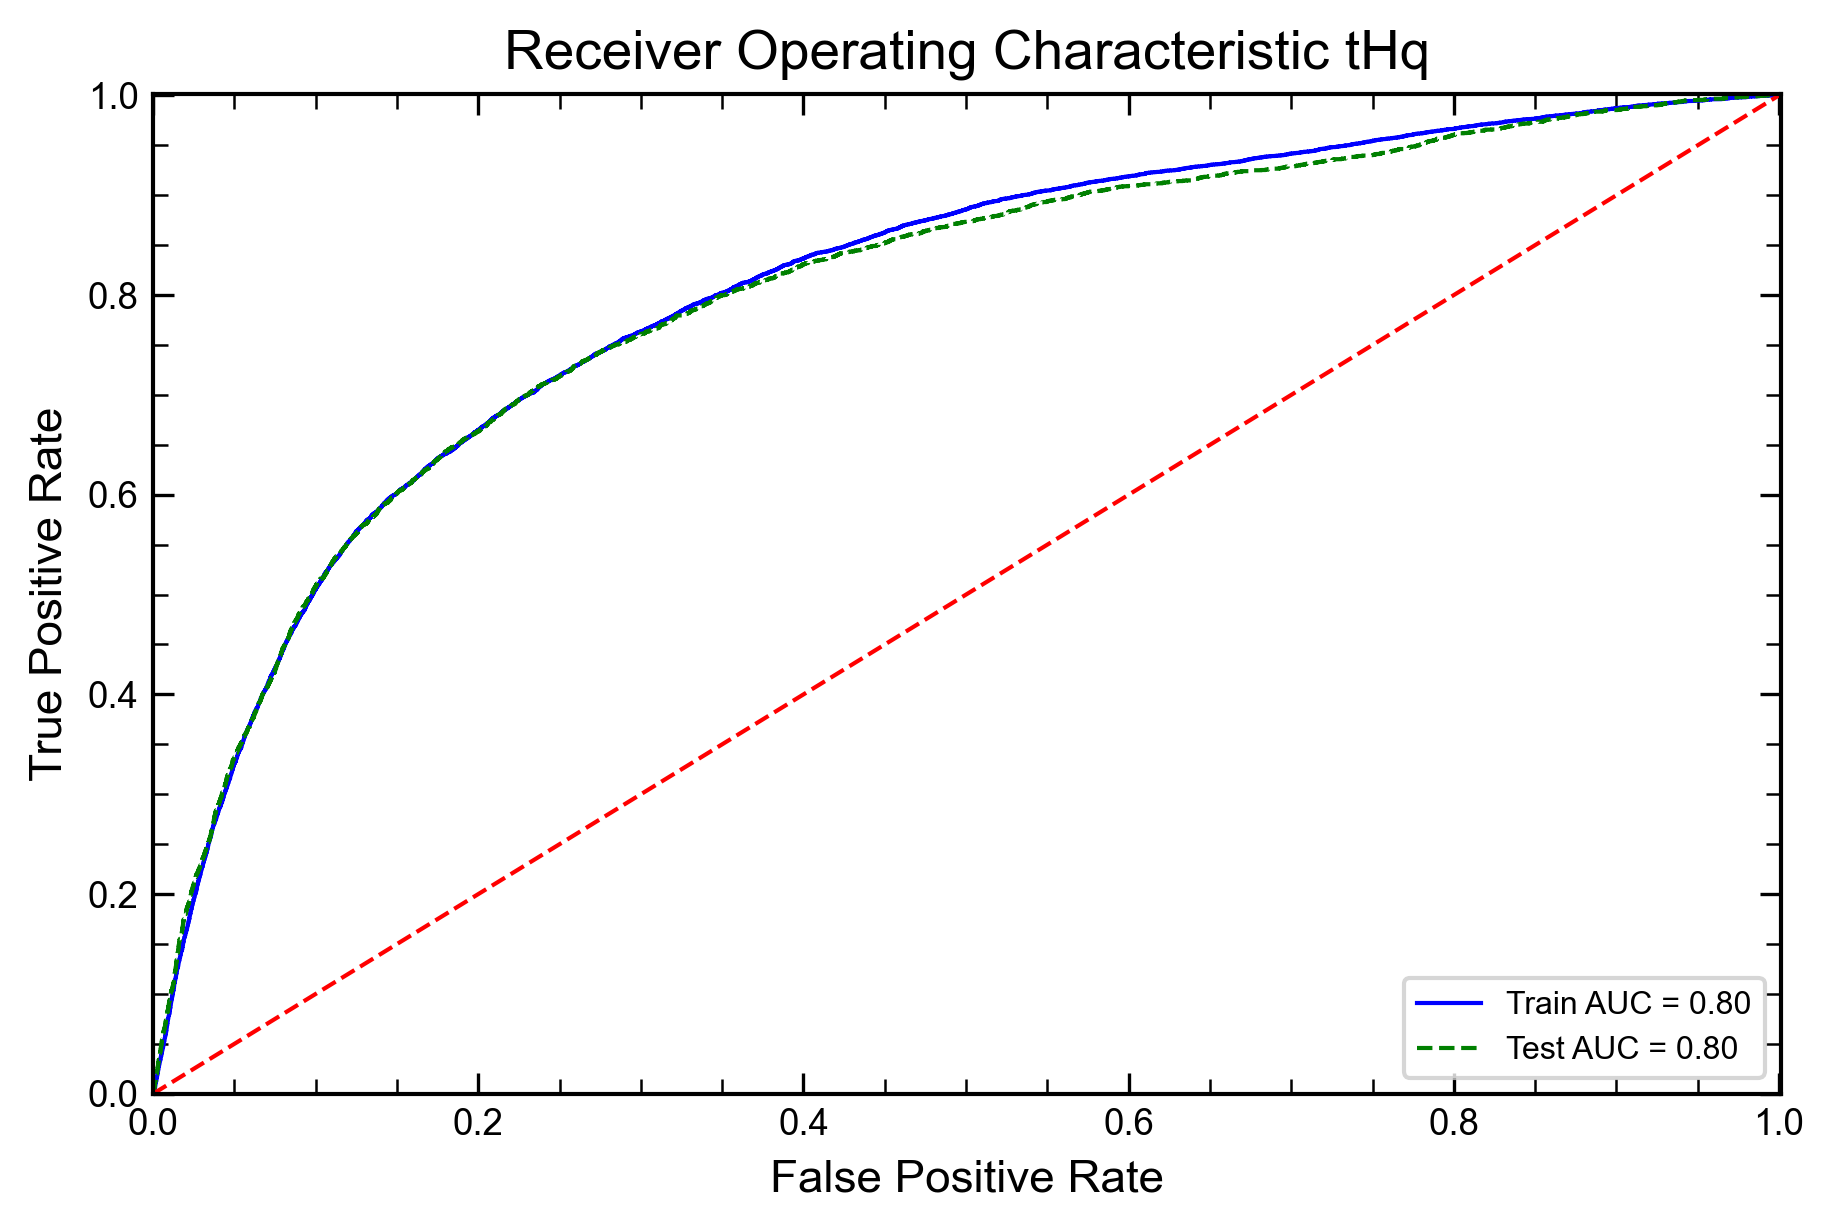
\includegraphics[width=0.8\textwidth]{lephad_ROC}    
            \end{figure}
            \vspace{-0.35cm}
            \begin{figure}
                \centering
                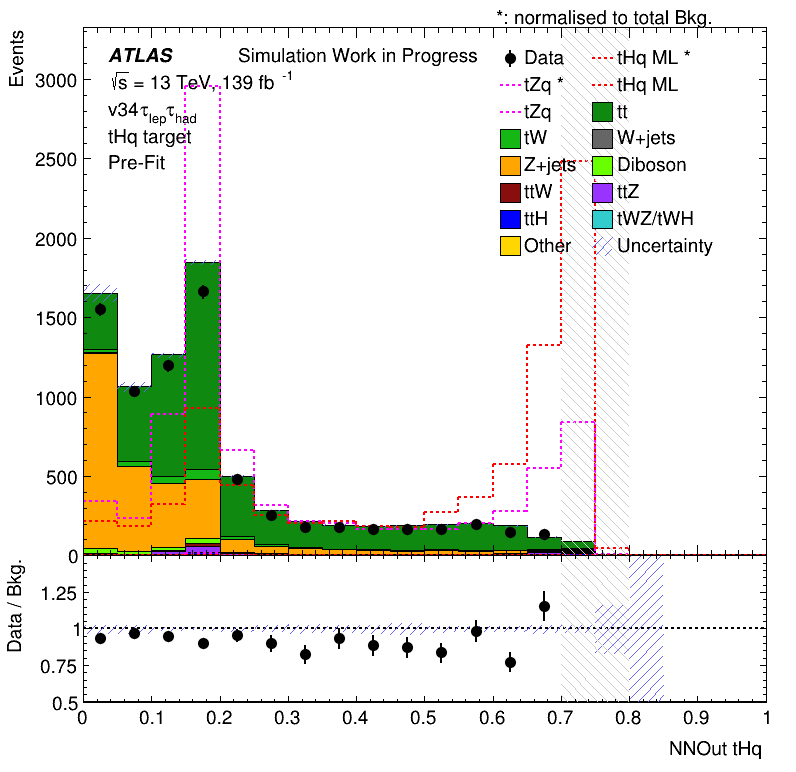
\includegraphics[width=0.8\textwidth]{lephad_2}    
            \end{figure}
        \end{column}
        \begin{column}{0.5\textwidth}
            \begin{block}{Setup}
                \begin{itemize}
                    \item Optimisation: Evolutionary + grid search
                    \item Model: Categorical (Treating \tZq separately)
                    \item Variables: final state kinematics
                    \item Train on absolute, predict on full weights
                \end{itemize}
            \end{block}
            \vspace{-0.2cm}
            \begin{block}{Plans}
               \begin{itemize}
                   \item Rerun the optimisation for v34
                   \item Rank and test variables
               \end{itemize} 
            \end{block}
        \end{column}
    \end{columns}
\end{frame}

\begin{frame}{Dileptau S/B}
    \begin{columns}
        \begin{column}{0.5\textwidth}
            \begin{figure}
                \centering
                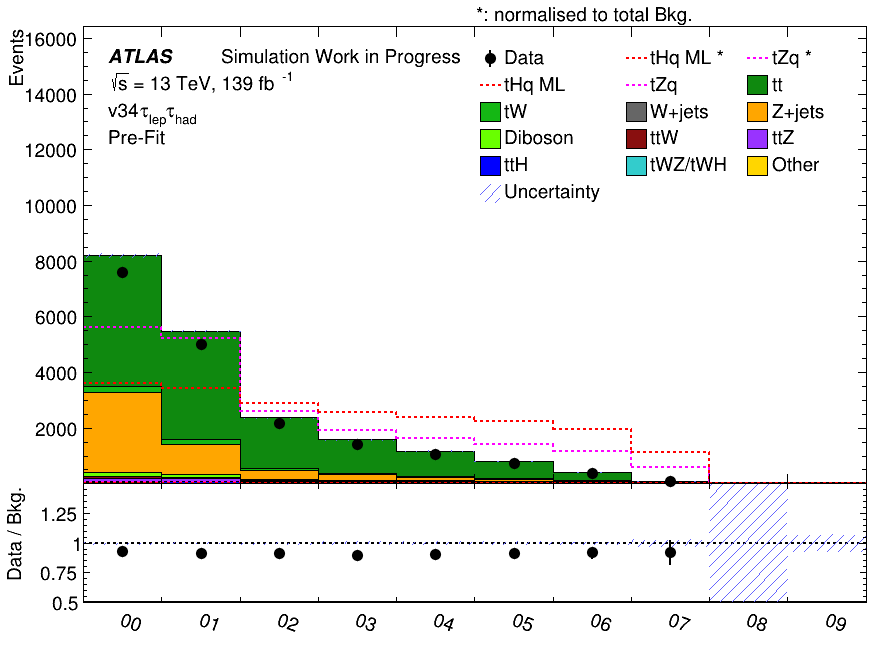
\includegraphics[width=\textwidth]{lephad_cutflow}
            \end{figure}
        \end{column}
        \begin{column}{0.5\textwidth}
            \begin{figure}
                \centering
                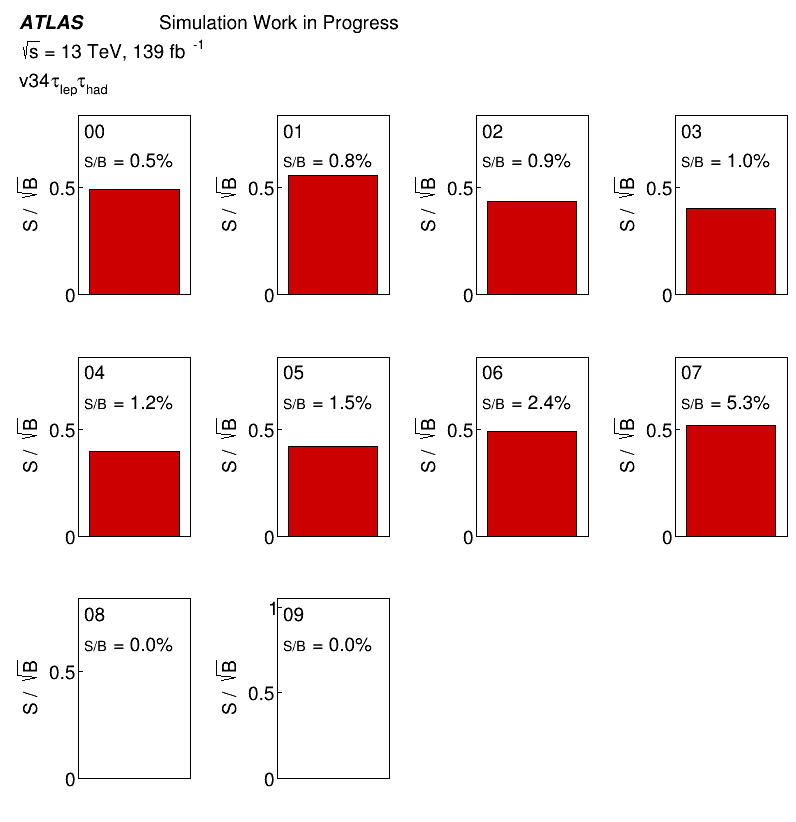
\includegraphics[width=\textwidth]{NN_sb}
            \end{figure}
        \end{column}
    \end{columns}
\end{frame}

\begin{frame}{Dileptau BDT}
    \begin{figure}
        \centering
        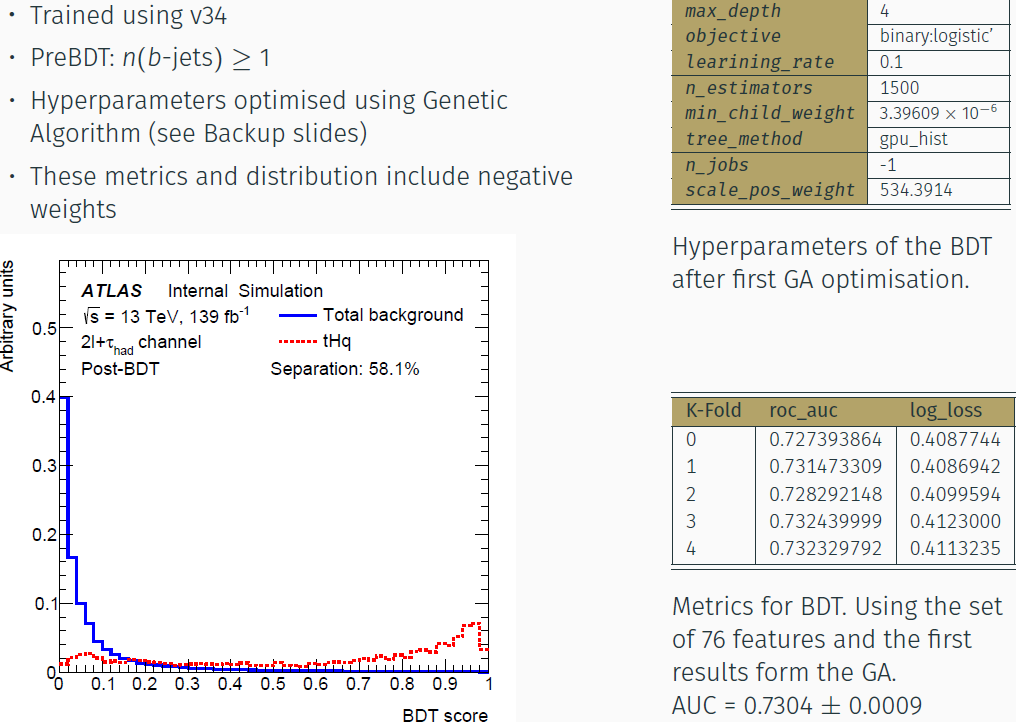
\includegraphics[width=0.9\textwidth]{BDT1}
    \end{figure}
\end{frame}

\begin{frame}{Dileptau BDT}
    \begin{figure}
        \centering
        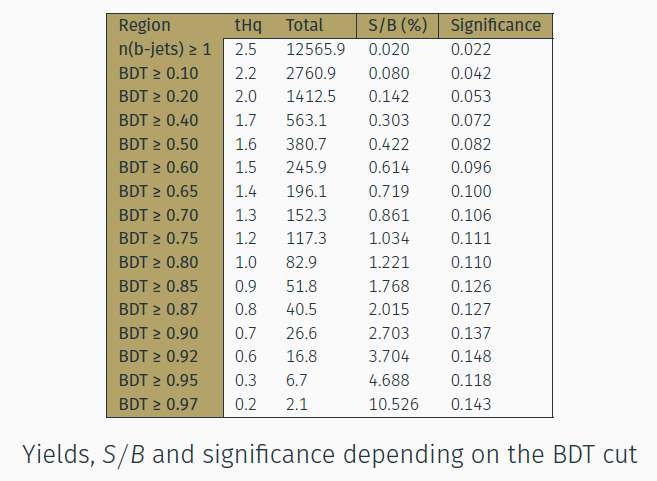
\includegraphics[width=0.9\textwidth]{BDT2}
    \end{figure}
\end{frame}

\begin{frame}{Dileptau BDT}
    \begin{itemize}
        \item BDT not using categorical approach
        \item \tZq separation is still quite good
    \end{itemize}
    \begin{figure}
        \centering
        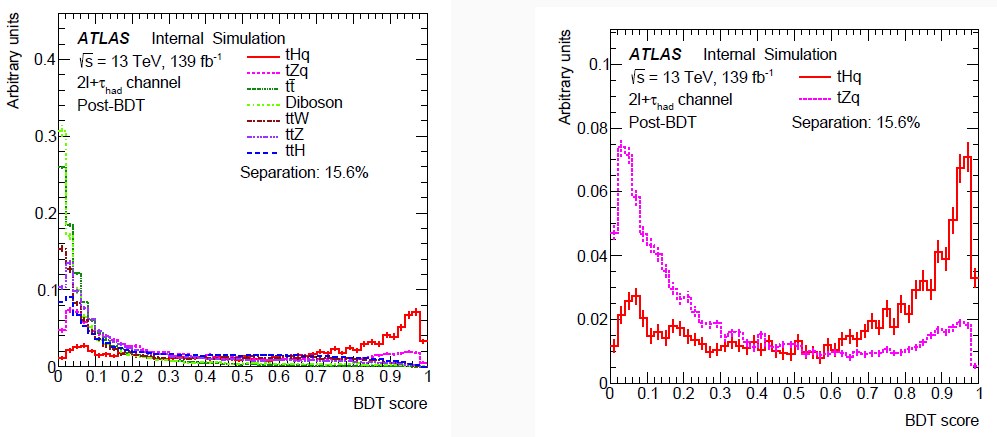
\includegraphics[width=0.9\textwidth]{BDT3}
    \end{figure}
\end{frame}
